\documentclass{beamer}
% Language/Font package
\usepackage[utf8]{inputenc}
\usepackage[francais]{babel}
\usepackage[T1]{fontenc}

% Base package
\usepackage{graphicx}
\usepackage{color}
\usepackage{listings}
\usepackage{hyperref}

% Configuration
\definecolor{ligthYellow}{RGB}{255,255,229}

\lstset{
language=bash,
numbers=left,
numberstyle=\small,
numbersep=8pt,
basicstyle=\small\ttfamily,
tabsize=4,
showspaces=false,
showstringspaces=false,
stringstyle=\color{red}\ttfamily,
commentstyle=\color{green}\ttfamily,
breaklines=true,
frame = single,
framexleftmargin=15pt,
backgroundcolor=\color{ligthYellow}}

% Theme https://github.com/matze/mtheme
\usetheme[progressbar=frametitle]{metropolis}

% Title
\title{Présentation Git}
\subtitle{Un outil de collaboration puissant}
\date{\today}
\author{Denis Pettens \and Pablo Gonzalez Alvarez}
\institute{Louvain-li-Nux}
\titlegraphic{\hfill
\includegraphics[height=2cm]{img/logo.png}}

\begin{document}

\maketitle

\begin{frame}{Table des matières}

\setbeamertemplate{section in toc}[sections numbered]
\tableofcontents[hideallsubsections]

\end{frame}

\section{Introduction}

\begin{frame}{Gérer un projet}
Comment gérez-vous actuellement un projet ?

\begin{itemize}
    \item L'envoyer à travers un message sur Facebook, ... (\textbf{Très mauvaise idée})
    \item L'envoyer par mail (\textbf{Un peu moins})
    \item Utiliser une Dropbox, Google Drive, ... (\textbf{Déjà mieux mais toujours risqué ou manque de fonctionalités})
\end{itemize}

Solution : Utiliser un \textbf{VCS}
\end{frame}

\begin{frame}{Monsieur, c'est quoi Git?}
\begin{itemize}
    \item \texttt{Git} a été créé en 2005 par \textbf{Linus Torvalds} (auteur du kernel \texttt{Linux});
    \item Il est le logiciel de gestion de versions décentralisé (\textbf{VCS}) le plus utilisé au monde en 2016;
    \item Il permet donc de suivre dans le temps l'avancement d'un projet de son début à sa fin;
    \item Il garde en mémoire tout ce que vous avez fait un jour dans votre projet et permet de les éditer facilement;
    \item ... \footnote{Tiré en partie du site (\url{https://git-scm.com})}
\end{itemize}
\end{frame}

\begin{frame}{Pourquoi l'utiliser?}
\begin{itemize}
    \item Le plus connu et utilisé (communauté très présente);
    \item Vitesse;
    \item Conception simple;
    \item Facile d'utilisation mais aussi très puissant;
    \item Support pour les développements non linéaires (milliers de branches parallèles);
    \item Complètement distribué;
    \item Capacité à gérer efficacement des projets d'envergure tels que le noyau Linux (vitesse et compacité des données).\footnote{Tiré en partie du site (\url{https://git-scm.com})}
\end{itemize}
\end{frame}

\begin{frame}{GitKraken}
\begin{itemize}
    \item \texttt{git} ne possède pas d'interface graphique, tout se fait en ligne de commande;
    \item Simple d'utilisation;
    \item Idéale pour avoir une vue globale de son projet;
    \item Cross-plaform;
    \item Malheureusement, il n'est pas Libre.
\end{itemize}

\textbf{Autres alternatives} : \texttt{gitg}, \texttt{GitHub Desktop}, \texttt{SourceTree}, ...
\end{frame}

\begin{frame}{GtiKraken : Image}
\begin{figure}
    \centering
    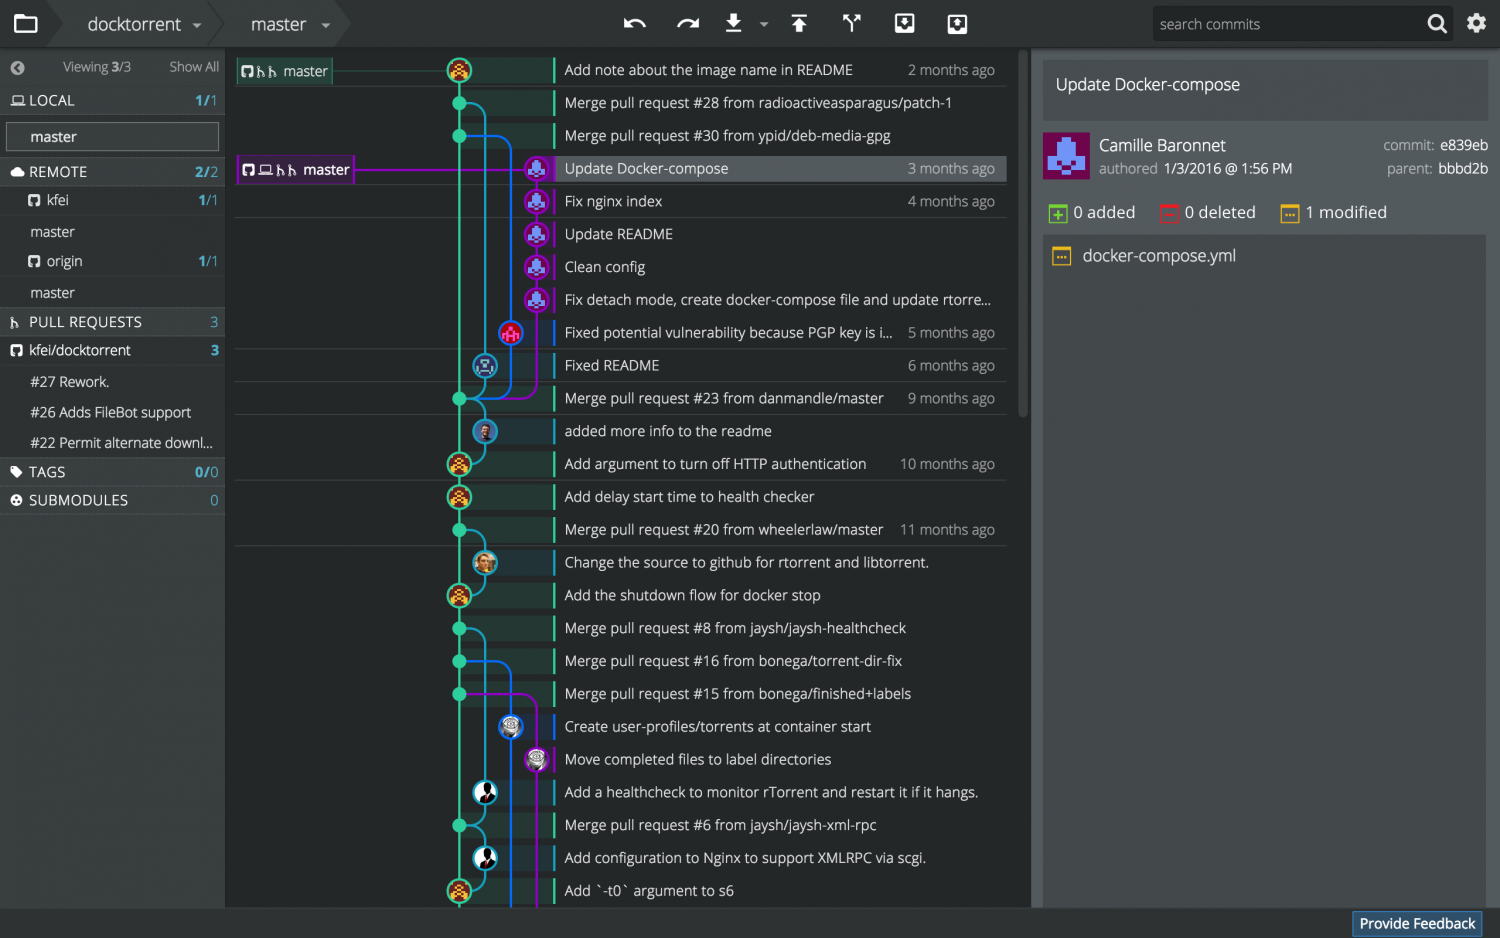
\includegraphics[height=6cm]{img/gitkraken.png}
    \caption{Tiré de \url{https://www.camillebaronnet.fr/blog/fr/gitkraken-enfin-outil-visuel-moderne-pour-git}}
\end{figure}
\end{frame}

\section{Instalation et configuration}
\begin{frame}{Installer Git et GiKraken}

\textbf{Git}
\begin{itemize}
\item \textbf{Ubuntu} : \lstinline{sudo apt-get install git}
\item \textbf{OS X} : \url{https://sourceforge.net/projects/git-osx-installer/}
\item \textbf{Windows} : \url{https://git-for-windows.github.io/}
\end{itemize}

\textbf{GitKraken}
\begin{itemize}
\item \textbf{Toutes plateformes} : \url{https://www.gitkraken.com/}
\end{itemize}
\end{frame}

\begin{frame}[fragile]
\frametitle{Configuration de base}

Git a besoin de deux informations de base sur vous pour pouvoir travailler efficacement :

\begin{itemize}
\item \textbf{Nom et Prénom}
\begin{lstlisting}
git config --global user.name "Jules Dupont"
\end{lstlisting}

\item \textbf{Email}
\begin{lstlisting}
git config --global user.email "jules.dupont@email.fr"
\end{lstlisting}
\end{itemize}

L'option \lstinline{--global} permet de configurer \texttt{git} pour tous vos autres projets sur votre PC.

GitKrakren demande de créer un compte par défaut pour pouvoir l'utiliser, ensuite il vous introduit rapidement sur son interface.
\end{frame}


  \end{frame}
  \section{Premier pas avec Git}
  \begin{frame}{git init}

  \end{frame}
  \begin{frame}{git add}

  \end{frame}
  \begin{frame}{git commit}

  \end{frame}
  \section{Manipuler l'historique}
  \section{Les branches}
  \section{Le travail en groupe}


\plain{Questions?}
\end{document}
